\begin{center}
\footnotesize
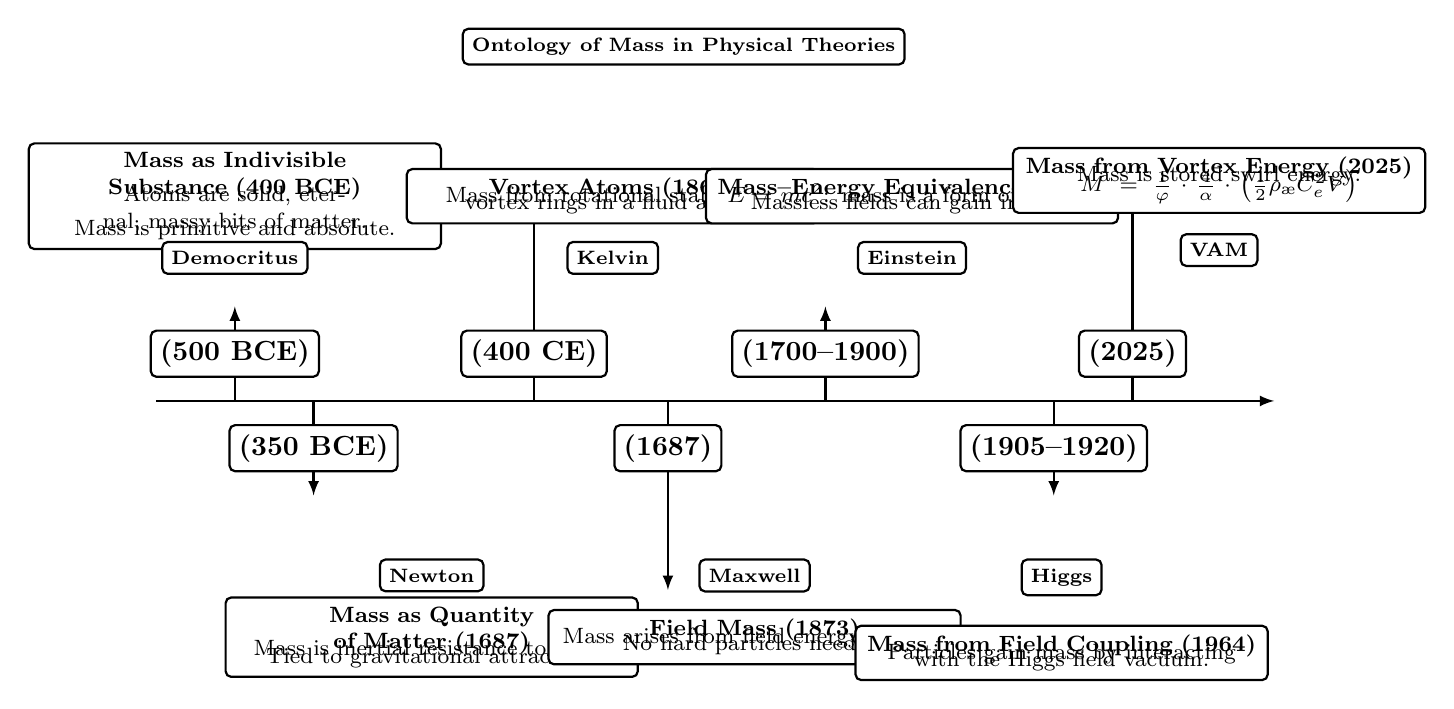
\begin{tikzpicture}[node distance=3.5cm, every node/.style={font=\footnotesize}, >=latex]


% Timeline base
\draw[->, thick] (-1,0) -- (13.2,0);

% Arrows above timeline (short, as requested)
\draw[->, thick] (0,0) -- (0,1.2);       % Pre-Socratics
\draw[->, thick] (3.8,0) -- (3.8,2.5);   % Augustine
\draw[->, thick] (7.5,0) -- (7.5,1.2);   % Einstein
\draw[->, thick] (11.4,0) -- (11.4,3.0); % VAM

% Arrows below timeline (short, as requested)
\draw[->, thick] (1.0,0) -- (1.0,-1.2);     % Plato/Aristotle
\draw[->, thick] (5.5,0) -- (5.5,-2.4);     % Newton
\draw[->, thick] (10.4,0) -- (10.4,-1.2);     % Leibniz/Mach

    %--- Root title cards (above timeline) ---
\node[draw, thick, rounded corners=2pt, fill=white, align=center, font=\bfseries ] at (0, .6)   {(500 BCE)};
\node[draw, thick, rounded corners=2pt, fill=white, align=center, font=\bfseries ] at (3.8, .6) {(400 CE)};
\node[draw, thick, rounded corners=2pt, fill=white, align=center, font=\bfseries ] at (7.5, .6) {(1700--1900)};
\node[draw, thick, rounded corners=2pt, fill=white, align=center, font=\bfseries ] at (11.4, .6){(2025)};

%--- Root title cards (below timeline) ---
\node[draw, thick, rounded corners=2pt, fill=white, align=center, font=\bfseries ] at (1.0,- .6) {(350 BCE)};
\node[draw, thick, rounded corners=2pt, fill=white, align=center, font=\bfseries ] at (5.5,- .6) {(1687)};
\node[draw, thick, rounded corners=2pt, fill=white, align=center, font=\bfseries ] at (10.4,- .6) {(1905--1920)};

% Label
\node[draw, thick, fill=white, rounded corners=2pt, font=\scriptsize] at (5.7,4.5) {\textbf{Ontology of Mass in Physical Theories}};

% Democritus (left)
\node[draw, rounded corners=2pt, thick, align=center, fill=white, text width=5cm] at (0,2.6) {
\textbf{Mass as Indivisible Substance (400 BCE)}  \\[-0.8em]
Atoms are solid, eternal, massy bits of matter.  \\[-0.8em]
Mass is primitive and absolute.
};

\node[above=1.6cm, draw, thick, fill=white, rounded corners=2pt, font=\scriptsize] at (0,0) {\textbf{Democritus}};

% Newton (below)
\node[draw, rounded corners=2pt, thick, align=center, fill=white, text width=5cm] at (2.5,-3.0) {
\textbf{Mass as Quantity of Matter (1687)}  \\[-0.8em]
Mass is inertial resistance to force.  \\[-0.8em]
Tied to gravitational attraction.
};

\node[below=2.0cm, draw, thick, fill=white, rounded corners=2pt, font=\scriptsize] at (2.5,0) {\textbf{Newton}};

% Kelvin (top)
\node[draw, rounded corners=2pt, thick, align=center, fill=white, text width=5cm] at (4.8,2.6) {
\textbf{Vortex Atoms (1867)}  \\[-0.8em]
Mass from rotational stability of  \\[-0.8em]
vortex rings in a fluid æther.
};

\node[above=1.6cm, draw, thick, fill=white, rounded corners=2pt, font=\scriptsize] at (4.8,0) {\textbf{Kelvin}};

% Maxwell (bottom)
\node[draw, rounded corners=2pt, thick, align=center, fill=white, text width=5cm] at (6.6,-3.0) {
\textbf{Field Mass (1873)}  \\[-0.8em]
Mass arises from field energy density.  \\[-0.8em]
No hard particles needed.
};

\node[below=2.0cm, draw, thick, fill=white, rounded corners=2pt, font=\scriptsize] at (6.6,0) {\textbf{Maxwell}};

% Einstein (top)
\node[draw, rounded corners=2pt, thick, align=center, fill=white, text width=5cm] at (8.6,2.6) {
\textbf{Mass–Energy Equivalence (1905)}  \\[-0.8em]
\( E = mc^2 \): mass is a form of energy.  \\[-0.8em]
Massless fields can gain inertia.
};

\node[above=1.6cm, draw, thick, fill=white, rounded corners=2pt, font=\scriptsize] at (8.6,0) {\textbf{Einstein}};

% Higgs (bottom)
\node[draw, rounded corners=2pt, thick, align=center, fill=white, text width=5cm] at (10.5,-3.2) {
\textbf{Mass from Field Coupling (1964)}  \\[-0.8em]
Particles gain mass by interacting  \\[-0.8em]
with the Higgs field vacuum.
};

\node[below=2.0cm, draw, thick, fill=white, rounded corners=2pt, font=\scriptsize] at (10.5,0) {\textbf{Higgs}};

% VAM (top right)
\node[draw, rounded corners=2pt, thick, align=center, fill=white, text width=5cm] at (12.5,2.8) {
\textbf{Mass from Vortex Energy (2025)}  \\[-0.8em]
Mass is stored swirl energy:  \\[-0.8em]
\( M = \frac{1}{\varphi} \cdot \frac{4}{\alpha} \cdot \left( \frac{1}{2} \rho_\text{\ae} C_e^2 V \right) \)
};

\node[above=1.7cm, draw, thick, fill=white, rounded corners=2pt, font=\scriptsize] at (12.5,0) {\textbf{VAM}};

\end{tikzpicture}
\captionof{figure}{Historical evolution of mass ontology: from indivisible substance to field energy and finally to vortex-stored rotational energy in the ætheric continuum of VAM.}
\end{center}